\section{Data}
The data I used for this task was provided by the VerSe`19: Large Scale Vertebrae Segmentation Challenge \cite{verse1, verse2}. The dataset consists of 80 CT scans of human spines, together with a vertebrae segmentation mask for every scan, both in the NIfTI format. The original dataset also includes .png overview of the segmentation and vertebrae centroid annotations (for another task of the challenge, which is out of the scope of this thesis). There are also additional 40 scans without annotations. For loading and working with NIfTI files, I used library NiBabel \cite{nibabel}.

The voxel-level vertebral annotations were created manually by two neurologists. The spine segmentation masks were derived by me from the vertebral masks.

\begin{figure}[ht]
    \centering
    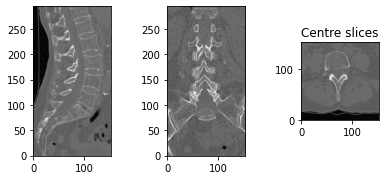
\includegraphics[width=250pt]{images/ct-sample.png}
    \caption[Sample data]{Saggital (side), coronal (frontal) and axial (horizontal) slices of a sample of the data}
    \label{fig:data-sample}
\end{figure}

\begin{figure}[ht]
    \centering
    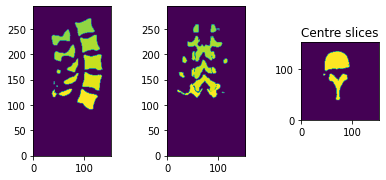
\includegraphics[width=250pt]{images/mask-sample.png}
    \caption{Vertebral segmentation mask of \ref{fig:data-sample}}
    \label{fig:mask-sample}
\end{figure}

\subsection{Spine}
Human spine consists of 24 vertebrae: C1-C7 (cervical spine), T1-T12 thoracic spine, L1-L5 lumbar spine. In very rare cases, an extra vertebrae L6 is present. Therefore, there are 26 classes in the data: background class [0] and vertebrae [C1-L6] which correspond to values [1-25] in the mask. Figure \ref{fig:vertebrae-annotations} shows annotations for [T2-L5].

\begin{figure}[ht]
    \centering
    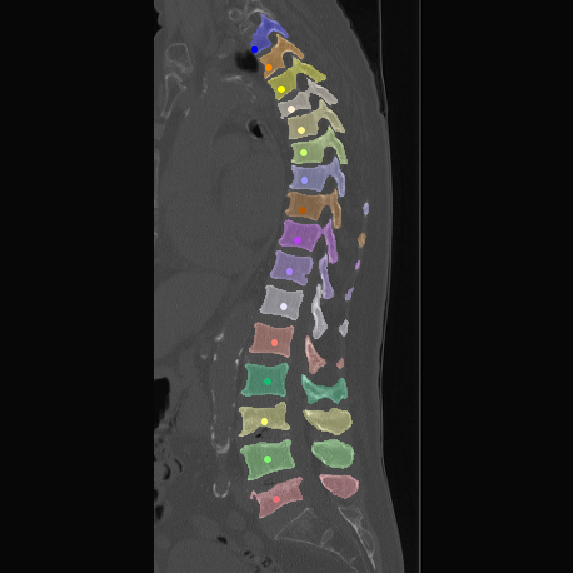
\includegraphics[width=150pt]{images/vertebrae-annotations.png}
    \caption{Vertebrae [T2-L5]}
    \label{fig:vertebrae-annotations}
\end{figure}

\subsection{Data characteristics}
One of the most important things about images when using neural networks is their size. In this dataset, images have various sizes in all dimensions, various ratios. The sizes range from as small as (57, 175, 175) to as big as (121, 915, 1189). Voxels do not store values typical for images (0-255), but attenuation values for the specific voxels. These vary all around the data set from -2290 (air) to 4106 (bones or metals). Voxels of the CT scans are also stored in various orientations: LAS, PIR, LPS and PSR.

Not all images contain the whole spine, usually it is some subset of vertebrae. This means, some of the vertebrae occur throughout the data set more often than others. [C1-C7] are underrepresented with less than 20 occurencies, [T1-T12] occur on average 35 times and the third group of vertebrae [L1-L5] is represented with more than 60 instances per vertebrae. The special L6 appears only in 2 scans from the whole dataset.

The dataset is imbalanced not only because of that, but also because different vertebrae cover different volumes. To put it easily, the background class is voxel-wise the most common class among the data. It accounts for more than 97\% of all voxels, the remaining 3\% is the spine. Also each vertebrae type accounts for less than 0.5\%. 

